%! Author = Frederik Bußmann
%! Date = 21.10.2021

% Preamble
\documentclass[ngerman,11pt]{article}

% Document packages and settings
%! Author = Frederik Bußmann
%! Date = 22.06.2023

% Packages
\usepackage[T1]{fontenc}
\usepackage[utf8]{inputenc}
\usepackage{babel}
\usepackage{csquotes}
\usepackage[nottoc]{tocbibind}
\usepackage[titles]{tocloft}
\usepackage[backend=biber,style=numeric,citestyle=ieee]{biblatex}

\usepackage[colorlinks,
    urlcolor = blue,
    linkcolor = black,
    citecolor = black,
    pdfpagelabels,
    pdfstartview = FitH,
    bookmarksopen = true,
    bookmarksnumbered = true,
    plainpages = false,
    hyperfootnotes = false,
    hypertexnames = false] {hyperref}

\usepackage{listings}
\usepackage{setspace}
\usepackage{graphicx}
\usepackage{adjustbox}
\usepackage{afterpage}
\usepackage[bottom=25.4mm,left=25.4mm,right=25.4mm,top=38mm]{geometry}

\usepackage[justification=centering]{caption}
\usepackage[noabbrev,nameinlink]{cleveref}
\usepackage[outputdir=/build/temp]{minted}
\usepackage[acronym,nomain,nonumberlist,nopostdot,nogroupskip,style=listdotted]{glossaries}

% Full-page background pictures
\usepackage{eso-pic}

% Decorations over headline
\usepackage{scrhack}
\usepackage[automark,headsepline]{scrlayer-scrpage}

%! Author = Frederik Bußmann
%! Date = 22.06.2023

\makeatletter
% Fix footnote second line indentation
\renewcommand{\@makefntext}[1]{%
    \begin{hangparas}{1.6em}{1}
        \noindent \makebox[1.2em]{\@makefnmark} #1
    \end{hangparas}
}

% Remove list of figures and tables titles
\renewcommand\listoffigures{%
    \@starttoc{lof}%
}
\renewcommand\listoftables{%
    \@starttoc{lot}%
}
\makeatother

% PDF Info
\hypersetup{
    pdfinfo={
        Author={Frederik Bußmann},
        Title={Konzeption und Entwicklung einer Continuous-Integration-Strategie für Kundenprojekte auf Basis der
        Shopware-Platform},
        Subject={Bachelor-Arbeit, Leitung Prof.\ Dr.-Ing.\ Martin Schulten},
        Keywords={},
    }
}
\title{Konzeption und Entwicklung einer Continuous-Integration-Strategie für Kundenprojekte auf Basis der
Shopware-Platform}
\author{Frederik Bußmann}
\date{Juli 2023}

% General settings
\setstretch{1.1}
\setlength{\parindent}{0pt}
\graphicspath{{/data}}

% Omit numbering of subsubsections
\setcounter{secnumdepth}{2}

% Add labels to bibliography entries to hyperlink them
\defbibenvironment{bibliography}
{\list
{\printtext[labelnumberwidth]{%
    \printfield{prefixnumber}%
    \printfield{labelnumber}}}
{\setlength{\labelwidth}{\labelnumberwidth}%
\setlength{\leftmargin}{\labelwidth}%
\setlength{\labelsep}{\biblabelsep}%
\addtolength{\leftmargin}{\labelsep}%
\setlength{\itemsep}{\bibitemsep}%
\setlength{\parsep}{\bibparsep}}%
\renewcommand*{\makelabel}[1]{\hss##1}}
{\endlist}
{\hypertarget{cite.\thefield{entrykey}}{\item}}

% Use et al. instead of u.a.
\DefineBibliographyStrings{ngerman}{
    andothers = {et\addabbrvspace al\adddot},
    urlseen = {aufgerufen am},
}

% Add bibliography
\addbibresource{config/references.bib}

% Blank page command
\newcommand\blankpage{\null\thispagestyle{empty}\newpage}

% Full-size background picture command
\newcommand\BackgroundPic{%
    \put(0,0){%
        \parbox[b][\paperheight]{\paperwidth}{%
            \vfill
            \centering
            
\includegraphics[width=\paperwidth,height=\paperheight,%
                keepaspectratio]{images/layout/background}%
            \vfill
        }}}

% Cleveref figure name settings
\crefname{figure}{Abbildung}{Abbildung}
\Crefname{figure}{Abbildung}{Abbildung}

% Glossary settings
\makeglossaries
%! Author = Frederik Bußmann
%! Date = 22.06.2023

\newacronym{ci}{CI}{Continuous Integration}

\newacronym{cd}{CD}{Continuous Deployment}

\newacronym{cde}{CDE}{Continuous Delivery}

\newacronym{ce}{CE}{Continuous Exploration}

\newacronym{ide}{IDE}{Integrated Development Environment}

\newacronym{api}{API}{Application Programming Interface}

\newacronym{cms}{CMS}{Content Management System}

\newacronym{vcs}{VCS}{Version Control System}

\newacronym{di}{DI}{Dependency Injection}

\newacronym{orm}{ORM}{Object-Relational Mapping}

\newacronym{npm}{NPM}{Node Package Manager}

\newacronym{yaml}{YAML}{YAML Ain't Markup Language}

\newacronym{ms}{MS}{Mutation Score}

\newacronym{msi}{MSI}{Mutation Score Indicator}

\newacronym{pr}{PR}{Pull Request}

\newacronym{mr}{MR}{Merge Request}

\newacronym{css}{CSS}{Cascading Style Sheets}

\newacronym{qa}{QA}{Quality Assurance}

\newacronym{cli}{CLI}{Command-Line Interface}

\newacronym{phpmd}{PHPMD}{PHP Mess Detector}

\newacronym{phpcs}{PHPCS}{PHP Code Sniffer}

\newacronym{pm}{PM}{Project Manager}

\newacronym{tty}{TTY}{Teletypewriter}

\newacronym{vm}{VM}{Virtual Machine}

\newacronym{os}{OS}{Operating System}

\newacronym{ui}{UI}{User Interface}

\renewcommand{\glsnamefont}[1]{\textbf{#1}}
\setlength{\glslistdottedwidth}{0.32\linewidth}

% List styling
\renewcommand{\labelitemii}{$\circ$}

% Footpartcite citation command
\DeclareCiteCommand{\footpartcite}[\mkbibfootnote]
{\usebibmacro{prenote}}
{%
    \hyperlink{cite.\thefield{entrykey}}{%
        \setunit{\addnbspace}%
        \printtext{Vgl.}%
        \setunit{\addnbspace}%
        \printnames{labelname}%
        \setunit{\labelnamepunct}%
        \printfield[citetitle]{title}%
        \newunit%
        \printfield{year}%
    }%
}
{\addsemicolon\space}
{\usebibmacro{postnote}}
% To cite: \footpartcite{example}

% Textpartcite citation command
\DeclareCiteCommand{\textpartcite}
{\usebibmacro{prenote}}
{%
    \hyperlink{cite.\thefield{entrykey}}{%
    \printnames{labelname}%
    \ (\printfield{year})%
}%
}
{\addsemicolon\space}
{\usebibmacro{postnote}}

% Caption cite command
\newcommand{\captioncite}[3][]{%
    \ifthenelse{\equal{#3}{}}{%
        \caption*{\fontsize{8pt}{6pt}\selectfont Quelle: \textpartcite{#1}}%
        \caption{#2}%
    }{%
        \caption*{\fontsize{8pt}{6pt}\selectfont Quelle: #1 \ifthenelse{\equal{#2}{}}{}{\textpartcite{#2}}}%
        \caption{#3}%
    }%
}

% Footnote size and spacing
\renewcommand{\footnotesize}{\scriptsize}
\setlength{\footnotesep}{0pt}
\setlength{\skip\footins}{0.5cm}


% Document content
\begin{document}
    % Title page
    \AddToShipoutPicture{\BackgroundPic}
    \pagenumbering{gobble}
    %! Author = Frederik Bußmann
%! Date = 22.06.2023

\begin{titlepage}
    \newgeometry{left=3.6cm,right=3.6cm,top=2.5cm,bottom=2.5cm}
        \adjustbox{valign=t}{
\includegraphics[width=0.5\textwidth]{images/layout/w-hs}}
        \hspace{2.16cm}
        \adjustbox{valign=t,raise=-0.04cm}{
\includegraphics[width=0.35\textwidth]{images/layout/w-hs-text}}
        \vspace{1.6cm}

        \begingroup
        \fontsize{44pt}{46pt}\selectfont
        {\bfseries Bachelorarbeit}
        \endgroup

        \vskip 1.44cm

        \begingroup
        \fontsize{8pt}{6pt}\selectfont
        Titel der Arbeit // Title of Thesis
        \endgroup

        \vskip -0.1cm

        \begingroup
        \fontsize{12pt}{18pt}\selectfont
        {\bfseries Konzeption und Entwicklung einer Continuous-Integration-Strategie für Kundenprojekte auf Basis der
        Shopware-Platform\par}
        \endgroup
        \vskip -0.03cm

        \noindent\rule{14cm}{0.4pt}

        \vskip 0.1cm

        \begingroup
        \fontsize{8pt}{6pt}\selectfont
        Akademischer Abschlussgrad: Grad, Fachrichtung (Abkürzung) // Degree
        \endgroup

        \vskip 0.03cm

        \begingroup
        \fontsize{12pt}{14pt}\selectfont
        Bachelor of Science (B.Sc.)
        \endgroup

        \vskip -0.05cm

        \noindent\rule{14cm}{0.4pt}

        \vskip 0.13cm

        \begingroup
        \fontsize{8pt}{6pt}\selectfont
        Autorenname, Geburtsort // Name, Place of Birth
        \endgroup

        \vskip 0.03cm

        \begingroup
        \fontsize{12pt}{14pt}\selectfont
        Frederik Bußmann, Coesfeld
        \endgroup

        \vskip -0.05cm

        \noindent\rule{14cm}{0.4pt}

        \vskip 0.13cm

        \begingroup
        \fontsize{8pt}{6pt}\selectfont
        Studiengang // Course of Study
        \endgroup

        \vskip 0.03cm

        \begingroup
        \fontsize{12pt}{14pt}\selectfont
        Informatik.Softwaresysteme
        \endgroup

        \vskip -0.05cm

        \noindent\rule{14cm}{0.4pt}

        \vskip 0.13cm

        \begingroup
        \fontsize{8pt}{6pt}\selectfont
        Fachbereich // Department
        \endgroup

        \vskip 0.03cm

        \begingroup
        \fontsize{12pt}{14pt}\selectfont
        Wirtschaft und Informationstechnik
        \endgroup

        \vskip -0.05cm

        \noindent\rule{14cm}{0.4pt}

        \vskip 0.13cm

        \begingroup
        \fontsize{8pt}{6pt}\selectfont
        Erstprüferin/Erstprüfer // First Examiner
        \endgroup

        \vskip 0.03cm

        \begingroup
        \fontsize{12pt}{14pt}\selectfont
        Prof.\ Dr.-Ing.\ Martin Schulten
        \endgroup

        \vskip -0.05cm

        \noindent\rule{14cm}{0.4pt}

        \vskip 0.13cm

        \begingroup
        \fontsize{8pt}{6pt}\selectfont
        Zweitprüferin/Zweitprüfer // Second Examiner
        \endgroup

        \vskip 0.03cm

        \begingroup
        \fontsize{12pt}{14pt}\selectfont
        Martin Knoop
        \endgroup

        \vskip -0.05cm

        \noindent\rule{14cm}{0.4pt}

        \vskip 0.13cm

        \begingroup
        \fontsize{8pt}{6pt}\selectfont
        Abgabedatum // Date of Submission
        \endgroup

        \vskip 0.03cm

        \begingroup
        \fontsize{12pt}{14pt}\selectfont
        31.08.2023
        \endgroup

        \vskip -0.05cm

        \noindent\rule{14cm}{0.4pt}
    \restoregeometry
\end{titlepage}
\clearpage


    % Statement
    %! Author = Frederik Bußmann
%! Date = 22.06.2023

\thispagestyle{empty}
\newgeometry{left=3.6cm,right=3.6cm,top=8.8cm,bottom=2.5cm}
    \begingroup
        \fontsize{18pt}{20pt}\selectfont
        {\bfseries Eidesstattliche Versicherung}
    \endgroup

    \vskip 0.8cm

    \begingroup
        \fontsize{12pt}{18pt}\selectfont
        Bußmann, Frederik
    \endgroup

    \vskip -0.35cm

    \noindent\rule{14.4cm}{0.4pt}

    \vskip -0.2cm

    \begingroup
        \fontsize{8pt}{6pt}\selectfont
        Name, Vorname // Name, First Name
    \endgroup

    \vskip 0.6cm
    \begingroup
        \fontsize{10.5pt}{11.5pt}\selectfont
        Ich versichere hiermit an Eides statt, dass ich die vorliegende Abschlussarbeit mit dem Titel
    \endgroup

    \vskip 0.3cm

    \begingroup
        \fontsize{12pt}{18pt}\selectfont
        {\bfseries Konzeption und Entwicklung einer Continuous-Integration-Strategie für Kundenprojekte auf Basis der
        Shopware-Platform}
    \endgroup

    \vskip 0.3cm

    \begingroup
        \fontsize{10.5pt}{11.5pt}\selectfont
        selbstständig und ohne unzulässige fremde Hilfe erbracht habe.
        Ich habe keine anderen als die angegebenen Quellen und Hilfsmittel benutzt sowie wörtliche und sinngemäße
        Zitate kenntlich gemacht.
        Die Arbeit hat in gleicher oder ähnlicher Form noch keiner Prüfungsbehörde vorgelegen.
    \endgroup

    \vskip 0.8cm
    {\fontsize{12pt}{18pt}\selectfont
    Stadtlohn, den}

    \vskip -0.35cm

    \noindent\rule{14.4cm}{0.4pt}

    \vskip -0.2cm

    \begingroup
        \fontsize{8pt}{6pt}\selectfont
        Ort, Datum, Unterschrift // Place, Date, Signature
    \endgroup
\restoregeometry
\clearpage

    \ClearShipoutPicture

    % Empty page
    \afterpage{\blankpage}
    \clearpage

    % Abstract
    \thispagestyle{empty}
    \newgeometry{left=25.4mm,right=25.4mm,top=25.4mm,bottom=25.4mm}
    %! Author = Frederik Bußmann
%! Date = 22.06.2023

\section*{Abstract} \label{sec:00-abstract}

% @TODO: Text zu Ende schreiben

Das Ziel dieser Bachelorarbeit ist die Erarbeitung eines geeigneten Konzepts für das Einbinden von
Continuous-Development-Techniken in Shopware-Projekten.
Insbesondere die Praktiken und Methoden der Continuous Integration (\acrshort{ci}) werden im Verlauf der Arbeit
untersucht und erläutert.
...

\clearpage

    \restoregeometry

    % Table of contents
    \pagenumbering{Roman}
    \setcounter{page}{1}
    \tableofcontents
    \clearpage

    % Acronyms
    \addtocontents{toc}{\protect\setcounter{tocdepth}{0}}
    \printglossary[title={Abkürzungsverzeichnis},toctitle=ABKÜRZUNGSVERZEICHNIS]
    \addtocontents{toc}{\protect\setcounter{tocdepth}{2}}
    \clearpage

    % List of figures
    \addtocontents{toc}{\protect\setcounter{tocdepth}{0}}
    \listoffigures
    \addtocontents{toc}{\protect\setcounter{tocdepth}{2}}
    \clearpage

    % Document content
    \pagenumbering{arabic}
    \setcounter{page}{1}
    %! Author = Frederik Bußmann
%! Date = 22.06.2023

\section{Einleitung} \label{sec:01-introduction}

Im Rahmen dieser Arbeit werden verschiedene Aspekte betrachtet, um ein Konzept für das Einbinden von
Continuous Integration (\acrshort{ci}) in Shopware-basierten Projekten zu erarbeiten.
Shopware bietet als eine führende E-Commerce-Plattform und eine der bevorzugten Online-Shop-Lösungen in
Deutschland\footpartcite{shopware-usage-chart} eine solide Grundlage für Unternehmen, um im digitalen Raum
erfolgreich zu agieren.
Durch die gezielte Implementierung von CI-Praktiken in solchen Projekten kann der Entwicklungszyklus effizienter
gestaltet und die Qualität des Endprodukts gesteigert werden.
Dies unterstützt Unternehmen dabei, ihre Wettbewerbsfähigkeit zu erhöhen und eine agile und reaktionsschnelle
Entwicklungsumgebung zu etablieren.

\subsection{Motivation} \label{subsec:01-introduction-1}

In der heutigen schnelllebigen digitalen Welt ist die Fähigkeit, qualitativ hochwertige Softwareprodukte schnell auf den
Markt zu bringen nicht nur wünschenswert, sondern oft entscheidend für den Geschäftserfolg.
Die E-Commerce-Branche, geprägt durch ihre intensive Wettbewerbsdynamik, erfordert von Unternehmen eine kontinuierliche
Anpassung und Innovation, um im Markt bestehen zu können.
Hierbei nimmt die Effizienz und Effektivität der eingesetzten Softwareentwicklungsmethoden eine zentrale Rolle ein.
Um eine möglichst reaktionsschnelle und effektive Umgebung für Entwicklerteams in Shopware-basierten Projekten zu
schaffen, können Methodiken des Continuous-Software-Engineering verwendet werden.
Die Entwicklung einer robusten, jedoch flexiblen\ \acrshort{ci}-Strategie ist im Hinblick auf sich ständig
weiterentwickelnder Technologien und variierender Anforderungen besonders wichtig für die Sicherstellung der
Softwarequalität und wird in Zukunft immer relevanter.

\subsection{Zielsetzung} \label{subsec:01-introduction-2}

Die Entwicklung einer Continuous-Integration-Strategie für auf Shopware basierende Kundenprojekte ist das primäre Ziel
dieser Arbeit.
Die Strategie soll dazu beitragen, die Qualität der Software zu verbessern, die Effizienz des Entwicklungsprozesses zu
steigern und letztendlich die Kundenzufriedenheit zu erhöhen.
Die nachfolgend definierten Ziele $Z_n$ dienen als Leitfaden für die Konzeption und Entwicklung der
\acrshort{ci}-Strategie und stellen die geschäftsseitigen Anforderungen von Unternehmen in der E-Commerce-Branche an den
Entwicklungsprozess mit Shopware dar:

\begin{itemize}
    \item {
        \textbf{$Z_1$ Hohe Entwicklungsgeschwindigkeit}\par
        Die Einführung einer umfangreichen \acrshort{ci}-Strategie soll die Effizienz der Softwareentwicklungsteams
        verbessern und die Zeit bis zum Produkt-Release senken.
        Eine hohe Entwicklungsgeschwindigkeit sorgt für eine schnellere Auslieferung neuer Features und Fehlerbehebungen
        und somit zu einer niedrigeren Wartezeit für Kunden.
    }

    \item {
        \textbf{$Z_2$ Niedrige Fehlerrate}\par
        \acrshort{ci} soll dazu beitragen, Fehler frühzeitig im Entwicklungsprozess erkennen und beheben zu können, was
        die Qualität des Endprodukts verbessert.
        Die Stabilität und Qualität der Ausgelieferten Anwendung wirkt sich durch weniger Ausfälle und eine
        niedrigere Support-Zeit auf die Zufriedenheit von Kunden aus.
    }

    \item{
        \textbf{$Z_3$ Kontinuierliche Auslieferung neuer Software}\par
        Die \acrshort{ci}-Strategie und die damit verbundenen Prozesse die sich für Entwicklerteams ergeben, sollen
        zu einer anpassbaren Entwicklungsumgebung führen.
        Diese Umgebung soll durch kontinuierliche Weiterentwicklung an die ständig wechselenden Anforderungen der
        modernen Softwareentwicklung angepasst werden können, was die Wettbewerbsfähigkeit fördert.
    }
\end{itemize}

Bei der Konzeption sollen diese Ziele verfolgt und die Maßnahmen der zu erarbeiteten \acrshort{ci}-Strategie
dementsprechend ausgerichtet werden.
Die Strategie soll dabei nicht nur die technischen Aspekte von Continuous Integration berücksichtigen, sondern auch die
organisatorischen Veränderungen, die mit der Einführung von\ \acrshort{ci} einhergehen.
Darüber hinaus soll die Strategie flexibel genug sein, um sich an zukünftige Veränderungen und Entwicklungen anpassen
zu können.

\subsection{Struktur der Arbeit} \label{subsec:01-introduction-3}

Im Laufe dieser Arbeit wird eine \acrshort{ci}-Strategie für Shopware-basierte Kundenprojekte konzeptioniert und
entwickelt.
Die Arbeit ist in fünf Hauptabschnitte unterteilt, die jeweils unterschiedliche Aspekte des Prozesses abdecken.

\subsubsection{Fachlicher Hintergrund}

In diesem Abschnitt wird zunächst der theoretische Rahmen für die Arbeit festgelegt.
Dies umfasst eine Einführung in das Continuous-Software-Engineering und die Prinzipien und Praktiken von
Continuous Integration, sowie eine Übersicht über die Shopware-Plattform.
Der Abschnitt dient dazu, ein grundlegendes Verständnis für die Themen und Technologien zu schaffen, die in
der Arbeit behandelt werden.

\subsubsection{Analyse und Konzept}

Dieser Abschnitt befasst sich mit der Analyse der aktuellen Situation und der Entwicklung eines Konzepts für die
\acrshort{ci}-Strategie.
Dies beinhaltet die Identifizierung von Herausforderungen und Anforderungen, die Berücksichtigung von Best
Practices und die Ausarbeitung eines Plans für die Implementierung der Strategie.
Die Konzeptionierung stützt sich dabei auf die im vorherigen Abschnitt aufgezeigte Fachliteratur.
Der Abschnitt dient als Brücke zwischen Theorie und Praxis und stellt sicher, dass die entwickelte Strategie sowohl
fundiert als auch anwendbar ist.

\subsubsection{Umsetzung der \acrshort{ci}-Strategie}

In diesem Abschnitt wird die Umsetzung der \acrshort{ci}-Strategie als Fallbeispiel beschrieben.
Dies umfasst die Auswahl und Konfiguration der benötigten Tools, die Definition von Prozessen und Workflows,
die Implementierung von Automatisierungen und Tests sowie das automatisierte Ausliefern der Software.
Der Schwerpunkt liegt hierbei auf der praktischen Umsetzung des zuvor entwickelten Konzepts und dessen Integration in
reale Shopware-Projekte.

\subsubsection{Evaluierung}

Die Auswertung der implementierten \acrshort{ci}-Strategie wird im folgenden Abschnitt behandelt.
Dabei wird die umgesetzte Strategie im Hinblick auf die im fachlichen Hintergrund aufgezeigten Prinzipien
geprüft.
Die Ergebnisse dieser Evaluierung werden analysiert und interpretiert, um Rückschlüsse auf den Erfolg der
Strategie zu ziehen.

\subsubsection{Schlussfolgerung und Ausblick}

Der letzte Abschnitt fasst die Ergebnisse der Arbeit zusammen und es werden Schlussfolgerungen über die
\acrshort{ci}-Strategie und dessen Anwendbarkeit in Shopware-Projekten gezogen.
Darüber hinaus wird ein Ausblick auf mögliche, zukünftige Entwicklungen und Verbesserungen gegeben.
Dieser Abschnitt dient dazu, die Arbeit abzurunden und einen Ausblick auf weitere Forschungs- und
Entwicklungsarbeiten in diesem Bereich zu geben.

\clearpage


    % Bibliography
    \printbibliography[heading=bibintoc,title={Literaturverzeichnis}]
    \clearpage

    % Appendix
    %\setcounter{secnumdepth}{0}
    %%! Author = Frederik Bußmann
%! Date = 22.06.2023

\section{Anhang I: Übersicht der verwendeten CI-Tools} \label{sec:appendix-1}

In Kapitel\ \ref{subsec:04-implementation-2} wurden verschiedene\ \acrshort{ci}-Tools und Services vorgestellt, welche
für die Fallstudie zur Umsetzung der Strategie eingesetzt wurden.
Im Folgenden wird eine Übersicht der genutzten Tools und dessen Funktionen und Merkmale gegeben:

\subsection*{Version-Control-System und Pipeline-Runner}

\begin{itemize}
    \item {
        \textbf{GitLab}\par
        GitLab ist ein webbasierter Service für Versionierung mit dem\ \acrshort{vcs}\ \glqq Git\grqq.
        Es bietet alle verteilten Versionskontroll- und Quellcodeverwaltungsfunktionen von Git sowie einige zusätzliche
        Features.
        Dies umfasst zum Beispiel eine Zugriffskontrolle und mehrere Kollaborationsfunktionen wie Aufgabenverwaltung,
        Fehlerverfolgung und Feature-Anfragen für Projekte, sowie eine integrierte Wiki-Funktion für die
        Dokumentation.
        Der Service bietet außerdem \acrshort{ci}-Tools und Pipeline-Verwaltung an.
        Dieser wird unter einer Open-Source-Lizenz vertrieben und dessen Self-Managed-Version ermöglicht es,
        GitLab auf eigenen Servern zu installieren und zu verwalten.\footpartcite{gitlab}
    }

    \item {
        \textbf{GitLab CI/CD}\par
        GitLab CI/CD ist der Pipeline-Runner von GitLab und stellt eine eingebaute Pipeline-Lösung für das Ausführen von
        \acrshort{ci}- und \acrshort{cd}-Prozessen dar.
        Das Tool ist vollständig in GitLab integriert und verwendet eine Konfigurations-Datei innerhalb des
        Repositories, um die Phasen und Jobs der \acrshort{ci}-Pipelines zu definieren.
        Es bietet eine breite Palette von Funktionen, einschließlich der Parallelisierung von Jobs, Pipelines für
        unterschiedliche Branches und das Verwalten von Umgebungsvariablen.
        GitLab CI/CD kann auf eigenen Servern oder in der Cloud ausgeführt werden, und sowohl für bei GitLab, als auch
        für extern gehostete Repositorys verwendet werden, was es zu einer flexiblen Lösung macht.
        Die für das Ausführen der Pipeline benötigten Umgebungsvariablen, Passwörter und andere vertrauliche Daten
        können dabei in einer von GitLab zur Verfügung gestellten, sicheren Datenbank verwaltet werden.
        \footpartcite{gitlab-ci-cd}
    }
\end{itemize}

\subsection*{Software-Testing}

\begin{itemize}
    \item {
        \textbf{PHPUnit}\par
        PHPUnit ist ein weit verbreitetes Open-Source Unit-Testing-Framework, welches zum Erstellen von
        Unit-Tests in PHP-basierten Applikationen verwendet wird.
        Das Framework ermöglicht das Erstellen von Mocks und das Auswerten der Test-Coverage für das zu
        testende Projekt.
        \footpartcite{phpunit}
    }

    \item {
        \textbf{Infection}\par
        Infection ist eine Mutation-Testing-Library für PHP.
        Sie ändert den Quellcode automatisch und führt dann bestehende Tests erneut aus, um zu sehen, ob diese
        fehlschlagen.
        Wenn die Tests bestehen, obwohl der Code mutiert wurde, zeigt Infection diese Stellen im Code an, damit
        diese verbessert werden können.
        Die Library unterstützt die Integration mit PHPUnit und weiteren Testing-Tools.
        \footpartcite{infection}
    }

    \item {
        \textbf{Jest}\par
        Jest ist ein Javascript Testing-Framework und ermöglicht das Einbringen von Unit-Tests in
        JavaScript-basierten Applikationen.
        Ähnlich wie PHPUnit, unterstützt Jest das Erstellen von Mocks und bietet Funktionen zur Coverage an.
        Das Framework parallelisiert laufende Tests, um eine möglichst hohe Performance zu bieten.
        \footpartcite{jest}
    }

    \item {
        \textbf{Cypress}\par
        Cypress ist ein Framework für Webapplikationen, um Functional-Tests durchzuführen.
        Es ermöglicht das automatisierte Testen von Benutzerinteraktionen innerhalb einer Webapplikation in
        einem realen Browser.
        Cypress ermöglicht das Testen des Zusammenspiels des gesamten Projekts und kann zur automatisierung
        von Testfällen genutzt werden, bei denen normalerweise Nutzer-Interaktion erforderlich ist.
        \footpartcite{cypress}
        Shopware bietet eine eigene Test-Suite für System-Tests durch Cypress an.\footpartcite{shopware-cypress}
    }
\end{itemize}

\subsection*{Static-Code-Analysis}

\begin{itemize}
    \item {
        \textbf{PHP\_CodeSniffer}\par
        PHP\_CodeSniffer (\acrshort{phpcs}) ist ein Set aus zwei Kommandozeilen-Befehlen für das Analysieren von PHP-
        und JavaScript-Code und von Cascading Style Sheets (\acrshort{css}) nach einem gegebenen Coding-Standard und für
        das automatische Korrigieren von Abweichungen dieses Standards.
        Das Tool kann mit vorgegebenen und eigens erstellten oder angepassten Regelsätzen betrieben werden.
        \footpartcite{php-codesniffer}
    }

    \item {
        \textbf{PHP Mess Detector}\par
        PHP Mess Detector (\acrshort{phpmd}) ist eine Software die nach vorgegebenen Problemen und Unstimmigkeiten in
        PHP-Code sucht.
        Das Tool kann zum verhindern des Einführens von überflüssigen Variablen und Methoden, unoptimiertem Code und
        möglichen Fehlern in die Zielumgebung genutzt werden.
        \acrshort{phpmd} kann ergänzend zu Danger und \acrshort{phpcs} zur statischen Analyse von PHP-Code verwendet
        werden.\footpartcite{php-mess-detector}
    }

    \item {
        \textbf{PHPStan}\par
        PHPStan ist ein weiteres \acrshort{qa}-Tool für das statische Analysieren von PHP-Code.
        Es konzentriert sich auf die Erkennung von Fehlern, die im laufenden Betrieb zu Problemen führen können, wie
        z.B. Aufrufe von nicht existierenden Methoden, ungenutzte Variablen, usw.
        PHPStan kann in den Entwicklungsprozess integriert werden, um die Codequalität kontinuierlich zu verbessern.
        \footpartcite{phpstan}
    }

    \item {
        \textbf{Deptrac}\par
        Deptrac ist ein statisches Code-Analyse-Tool, das dabei hilft, die Architektur eines PHP-Projekts zu verstehen
        und zu überprüfen.
        Es stellt sicher, dass die Abhängigkeiten zwischen den Modulen eines Projekts den definierten Architekturregeln
        entsprechen.
        Deptrac kann in den Entwicklungsprozess integriert werden, um die Architektur des Projekts kontinuierlich zu
        überwachen und zu verbessern.\footpartcite{deptrac}
    }

    \item {
        \textbf{Eslint}\par
        ESLint ist ein statisches Tool zur Analyse von JavaScript-Code.
        Das Tool ist sehr anpassbar und kann für das Entwickeln mit verschiedenen Frameworks und Libraries genutzt
        werden.
        Viele \acrshort{ide}s unterstützen ESLint und zeigen Analyse-Resultate bereits bei der Entwicklung im Editor
        an.
        Das Tool unterstützt außerdem das automatische Beheben von bestimmten Syntax-Fehlern mit einem eingebauten
        Kommandozeilenbefehl.\footpartcite{eslint}
    }

    \item {
        \textbf{Danger JS}\par
        Danger ist ein statisches Analyse-Tool, welches direkt in \acrshort{vcs} angebunden werden kann.
        Das Tool läuft während des \acrshort{ci}-Prozesses und kann zur automatisierung von Code-Review-Aufgaben
        genutzt werden.
        Mit Danger können Warnungen und Fehler in der Pipeline geworfen werden, wenn geplante Integrationen zu
        groß werden, kein Changelog-Eintrag für Änderungen angelegt wurde, Abhängigkeiten nicht up-to-date sind und
        vieles mehr.
        Danger kann außerdem Job-Ergebnisse einer Pipeline in Form von Kommentaren in Merge-Requests hinterlegen,
        um Entwickler schneller über den Status des Projekts zu informieren.
        Die Software wird für die Programmiersprachen JavaScript, Ruby, Kotlin, Python und Swift angeboten.
        \footpartcite{danger-js}
    }

    \item {
        \textbf{License Checker}\par
        License checker sind Tools, die Lizenzen von Abhängigkeiten in einem Projekt überprüfen.
        Sie können dabei helfen, Lizenzprobleme bei Plugins und Erweiterungen von Drittanbietern zu identifizieren
        und zu vermeiden.
        Für das Prüfen von Composer- und\ \acrshort{npm}-Paketen existieren jeweils eigene PHP- und JavaScript-basierte
        Tools.
        \footpartcite{php-license-checker}\textsuperscript{,\ }\footpartcite{js-license-checker}
    }

    \item {
        \textbf{Security Checker / AuditJS}\par
        Security Checker sind Tools, die überprüfen, ob die in einem Projekt verwendeten Abhängigkeiten bekannte
        Sicherheitslücken aufweisen.
        Diese Tools können dabei helfen, Projekte kontinuierlich zu überwachen und sicher zu halten.
        Symfony bietet für das automatische Prüfen von Applikationen einen eigenen Security Checker.
        \footpartcite{symfony-security-checker}
        Darüber hinaus wurde zur Prüfung von JavaScript-Abhängigkeiten in der Fallstudie das JavaScript-basierte
        Sicherheitsprüfungs-Tool AuditJS verwendet.
        \footpartcite{audit-js}
    }
\end{itemize}

\clearpage

\subsection*{Deployment}

\begin{itemize}
    \item {
        \textbf{Deployer}\par
        Deployer ist ein PHP-basiertes Deployment-Tool, welches zur automatisierten Auslieferung von Software an
        verschiedene Umgebungen verwendet werden kann.
        Das Werkzeug bietet vordefinierte Setups für das Deployment verschiedener Services und weitere wichtige
        Features wie minimale Ausfallzeiten und die Möglichkeit, ausgelieferte Software auf einen früheren Stand
        zurückzurollen.
        \footpartcite{deployer}
        Shopware stellt eine Anleitung für das Einsetzen von Deployer in Projekten bereit, wobei auch die Nutzung mit
        GitLab CI/CD abgedeckt wird.
        \footpartcite{shopware-deployer}
    }
\end{itemize}

\clearpage

\section{Anhang II: Darstellung ausgeführter Pipelines} \label{sec:appendix-2}

Der für die Umsetzung der Fallstudie gewählte Pipeline-Runner GitLab CI/CD bietet eine Übersicht aller
Pipeline-Instanzen, die im Verlauf des Projekts durchgeführt wurden.
Neben dem Titel und der Art des Ausgangs-Branches der Pipeline wird hierbei auch der Status der Pipeline aufgezeigt:

\begin{figure}[H]
    \centering
    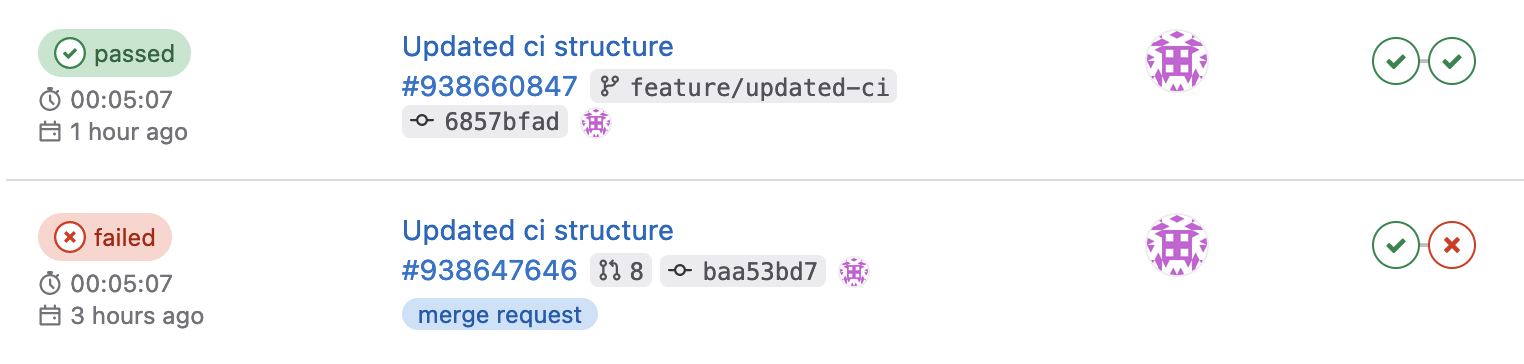
\includegraphics[width=\textwidth]{images/content/pipeline-overview}
    \captioncite[\hyperlink{cite.gitlab}{GitLab B.V.}]{}{Übersicht ausgeführter Pipelines in GitLab CI/CD}
    \label{fig:pipeline-overview}
\end{figure}

Abbildung\ \ref{fig:pipeline-overview} stellt einen Ausschnitt der Pipeline-Übersicht dar.
Es werden zwei verschiedene Pipelines angezeigt, wobei eine erfolgreich durchgeführt und die andere
aufgrund von Fehlern in einem der Jobs abgebrochen wurde.
Die fehlgeschlagene Pipeline wird dabei durch ein rotes X mit dem Schriftzug\ \glqq failed\grqq\ markiert, während die
erfolgreich durchgelaufene Pipeline einen grünen Haken und das Wort\ \glqq passed\grqq\ ausgibt.
\\\\
Navigiert man in der Pipeline-Auflistung von GitLab CI/CD zu der Detail-Ansicht einer der gezeigten Pipelines, werden
dessen Phasen und Jobs dargestellt.
Die hierbei angezeigten Jobs können entweder als erfolgreich oder fehlerhaft markiert werden:

\begin{figure}[H]
    \centering
    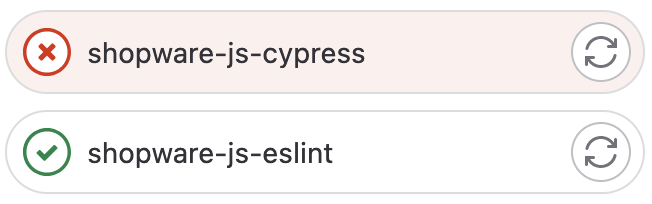
\includegraphics[width=0.5\textwidth]{images/content/job-status}
    \captioncite[\hyperlink{cite.gitlab}{GitLab B.V.}]{}{Status-Anzeige der Jobs einer Pipeline}
    \label{fig:job-status}
\end{figure}

In Abbildung\ \ref{fig:job-status} werden verschiedene Jobs aufgezeigt, welche jeweils einen unterschiedlichen Status
berichten.
Während der Job für das statische Code-Analyse-Tool Eslint erfolgreich durchgelaufen ist, wurde der Job zur
Durchführung von System-Tests durch Cypress abgebrochen.
Der erfolgreiche Job wird hierbei mit einem grünen Haken markiert, während der abgebrochene Job mit einem roten X
gekennzeichnet wurde.
\\\\
Neben den Job-Informationen werden in der Pipeline-Detail-Ansicht noch weitere Metriken, wie die Anzahl der in den Jobs
durchgeführten Tests oder die Dauer der gesamten Pipeline ausgegeben.
Eine Übersicht aller Jobs einer ausgewählten Pipeline wird in Abbildung\ \ref{fig:job-overview} angezeigt.
Diese implementiert die in Kapitel\ \ref{subsec:04-implementation-2} ausgewählten Tools der \acrshort{ci}-Strategie,
welche nach dem erfolgreichen Build-Job in der Testing-Phase der Pipeline stattfinden.
Jobs können in dieser Detail-Ansicht wiederholt und manche manuell angestoßen werden, wie zum Beispiel der
Deployment-Job für die Development-Umgebung, welcher in der Deployment-Phase der Pipeline ausführbar ist.
Dieser kann von den Entwicklern auf der Web-Oberfläche gestartet werden, um die gebaute und getestete Integration an die
hinterlegte Umgebung auszuliefern.

\begin{figure}[H]
    \centering
    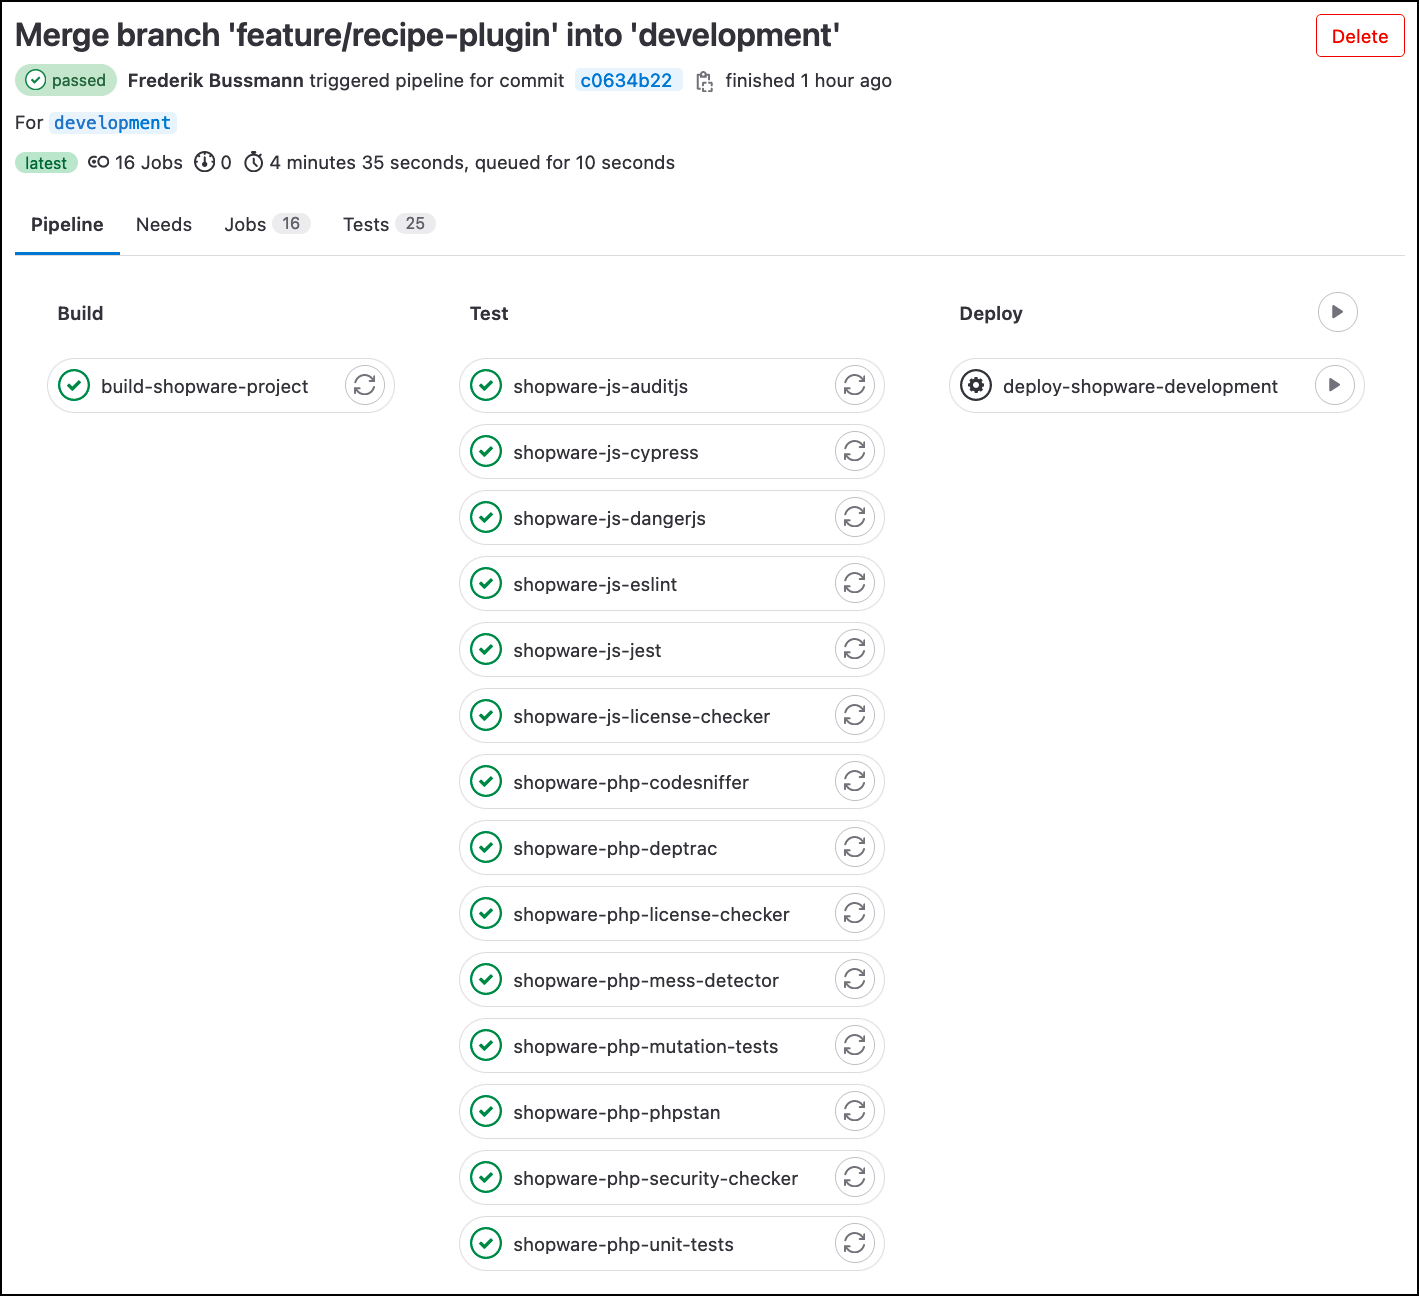
\includegraphics[width=\textwidth]{images/content/job-overview}
    \captioncite[\hyperlink{cite.gitlab}{GitLab B.V.}]{}{Detail-Ansicht einer durchgeführten Pipeline}
    \label{fig:job-overview}
\end{figure}

    %\clearpage
\end{document}
